%%%%%%%%%%%%%%%%%%%%%%%%%%%%%%%%%%%%%%%%%%%%%%%%%%%%%%%%%%%%%%%%%%%%%%%%%%%%%%%%%
% Template: Exam
%
% Por: Abrantes Araújo Silva Filho
%      abrantesasf@gmail.com
%
% Citação: Se você gostou deste template, por favor ajude a divulgá-lo mantendo
%          o link para meu repositório GitHub em:
%          https://github.com/abrantesasf/LaTeX
%%%%%%%%%%%%%%%%%%%%%%%%%%%%%%%%%%%%%%%%%%%%%%%%%%%%%%%%%%%%%%%%%%%%%%%%%%%%%%%%%




%%%%%%%%%%%%%%%%%%%%%%%%%%%%%%%%%%%%%%%%%%%%%%%%%%%%%%%%%%%%%%%%%%%%%%%%%%%%%%%%%
%%% Configura o tipo de documento, papel, tamanho da fonte e informações básicas
%%% para as proriedades do PDF/DVIPS e outras propriedades do documento
\RequirePackage{ifpdf}
\ifpdf
  % Classe, língua e tamanho da fonte padrão. Outras opções a considerar:
  %   draft
  %   onecolumn (padrão) ou twocolumn (OU usar o package multicol)
  %   fleqn com ou sem leqno (alinhamento à esquerda das fórmulas e dos números)
  %   oneside (padrão para article ou report) ou twoside (padrão para book)
  %   answers = imprime respostas para o gabarito
  \documentclass[pdftex, brazil, 12pt, oneside, addpoints]{exam}
\else
  % Classe, língua e tamanho da fonte padrão. Outras opções a considerar:
  %   draft
  %   onecolumn (padrão) ou twocolumn (OU usar o package multicol)
  %   fleqn com ou sem leqno (alinhamento à esquerda das fórmulas e dos números)
  %   oneside (padrão para article ou report) ou twoside (padrão para book)
  %   answers = imprime respostas para o gabarito
  \documentclass[brazil, 12pt, oneside, addpoints]{exam}
\fi


%%%%%%%%%%%%%%%%%%%%%%%%%%%%%%%%%%%%%%%%%%%%%%%%%%%%%%%%%%%%%%%%%%%%%%%%%%%%%%%%%
%%% Carrega pacotes iniciais necessários para estrutura de controle e para a
%%% criação e o parse de novos comandos
\usepackage{ifthen}
\usepackage{xparse}


%%%%%%%%%%%%%%%%%%%%%%%%%%%%%%%%%%%%%%%%%%%%%%%%%%%%%%%%%%%%%%%%%%%%%%%%%%%%%%%%%
%%% Configuração do tamanho da página, margens, espaçamento entrelinhas e, se
%%% necessário, ativa a indentação dos primeiros parágrafos.
\ifpdf
  \usepackage[pdftex]{geometry}
\else
  \usepackage[dvips]{geometry}
\fi
\geometry{a4paper, left=2.0cm, right=2.0cm, top=2.0cm, bottom=2.0cm}

\usepackage{setspace}
  \singlespacing
  %\onehalfspacing
  %\doublespacing


%%%%%%%%%%%%%%%%%%%%%%%%%%%%%%%%%%%%%%%%%%%%%%%%%%%%%%%%%%%%%%%%%%%%%%%%%%%%%%%%%
%%% Configurações de encoding, lingua e fontes:
\usepackage[T1]{fontenc}
\usepackage[utf8]{inputenc}
\usepackage{babel}

% Altera a fonte padrão do documento (nem todas funcionam em modo math):
%   phv = Helvetica
%   ptm = Times
%   ppl = Palatino
%   pbk = bookman
%   pag = AdobeAvantGarde
%   pnc = Adobe NewCenturySchoolBook
\renewcommand{\familydefault}{ppl}


%%%%%%%%%%%%%%%%%%%%%%%%%%%%%%%%%%%%%%%%%%%%%%%%%%%%%%%%%%%%%%%%%%%%%%%%%%%%%%%%%
%%% Configurações de cabeçalho e rodapé (não pode usar fancyhdr pois ocorre conflito):
\pagestyle{headandfoot}
\runningheadrule
\firstpageheader{}{}{}
\runningheader{Desafio 2: Matrizes}{}{Abril/2019}
\firstpagefooter{}{}{Página \thepage\ de \numpages}
\runningfooter{}{}{Página \thepage\ de \numpages}
\runningfootrule


%%%%%%%%%%%%%%%%%%%%%%%%%%%%%%%%%%%%%%%%%%%%%%%%%%%%%%%%%%%%%%%%%%%%%%%%%%%%%%%%%
%%% Carrega pacotes para referências cruzadas, citações dentro do documento,
%%% links para internet e outros.Configura algumas opções.
%%% Não altere a ordem de carregamento dos packages.
\usepackage{varioref}
\ifpdf
  \usepackage[pdftex]{hyperref}
    \hypersetup{
      % Informações variáveis em cada documento (MUDE AQUI!):
      pdftitle={Desafio 1: Matrizes},
      pdfauthor={Abrantes Araújo Silva Filho},
      pdfsubject={Matrizes e multiplicação de matriz por vetor},
      pdfkeywords={álgebra linear, matrizes, vetores, markov},
      pdfinfo={
        CreationDate={}, % Ex.: D:AAAAMMDDHH24MISS
        ModDate={}       % Ex.: D:AAAAMMDDHH24MISS
      },
      % Coisas que você não deve alterar se não souber o que está fazendo:
      unicode=true,
      pdflang={pt-BR},
      bookmarksopen=true,
      bookmarksnumbered=true,
      bookmarksopenlevel=5,
      pdfdisplaydoctitle=true,
      pdfpagemode=UseOutlines,
      pdfstartview=FitH,
      pdfcreator={LaTeX with hyperref package},
      pdfproducer={pdfTeX},
      pdfnewwindow=true,
      colorlinks=true,
      citecolor=green,
      linkcolor=red,
      filecolor=cyan,
      urlcolor=blue
    }
\else
  \usepackage{hyperref}
\fi
\usepackage{cleveref}
\usepackage{url}


%%%%%%%%%%%%%%%%%%%%%%%%%%%%%%%%%%%%%%%%%%%%%%%%%%%%%%%%%%%%%%%%%%%%%%%%%%%%%%%%%
%%% Carrega bibliotecas de símbolos (matemáticos, físicos, etc.), fontes
%%% adicionais, e configura algumas opções
\usepackage{amsmath}
\usepackage{amssymb}
\usepackage{amsfonts}
\usepackage{siunitx}
  \sisetup{group-separator = {.}}
  \sisetup{group-digits = {false}}
  \sisetup{output-decimal-marker = {,}}
\usepackage{bm}
\usepackage{cancel}
% Altera separador decimal via comando, se necessário (prefira o siunitx):
%\mathchardef\period=\mathcode`.
%\DeclareMathSymbol{.}{\mathord}{letters}{"3B}
  

%%%%%%%%%%%%%%%%%%%%%%%%%%%%%%%%%%%%%%%%%%%%%%%%%%%%%%%%%%%%%%%%%%%%%%%%%%%%%%%%%
%%% Carrega packages relacionados à computação
\usepackage{algorithm2e}
\usepackage{algorithmicx}
\usepackage{algpseudocode}
\usepackage{listings}
  \lstset{literate=
    {á}{{\'a}}1 {é}{{\'e}}1 {í}{{\'i}}1 {ó}{{\'o}}1 {ú}{{\'u}}1
    {Á}{{\'A}}1 {É}{{\'E}}1 {Í}{{\'I}}1 {Ó}{{\'O}}1 {Ú}{{\'U}}1
    {à}{{\`a}}1 {è}{{\`e}}1 {ì}{{\`i}}1 {ò}{{\`o}}1 {ù}{{\`u}}1
    {À}{{\`A}}1 {È}{{\'E}}1 {Ì}{{\`I}}1 {Ò}{{\`O}}1 {Ù}{{\`U}}1
    {ä}{{\"a}}1 {ë}{{\"e}}1 {ï}{{\"i}}1 {ö}{{\"o}}1 {ü}{{\"u}}1
    {Ä}{{\"A}}1 {Ë}{{\"E}}1 {Ï}{{\"I}}1 {Ö}{{\"O}}1 {Ü}{{\"U}}1
    {â}{{\^a}}1 {ê}{{\^e}}1 {î}{{\^i}}1 {ô}{{\^o}}1 {û}{{\^u}}1
    {Â}{{\^A}}1 {Ê}{{\^E}}1 {Î}{{\^I}}1 {Ô}{{\^O}}1 {Û}{{\^U}}1
    {œ}{{\oe}}1 {Œ}{{\OE}}1 {æ}{{\ae}}1 {Æ}{{\AE}}1 {ß}{{\ss}}1
    {ű}{{\H{u}}}1 {Ű}{{\H{U}}}1 {ő}{{\H{o}}}1 {Ő}{{\H{O}}}1
    {ç}{{\c c}}1 {Ç}{{\c C}}1 {ø}{{\o}}1 {å}{{\r a}}1 {Å}{{\r A}}1
    {€}{{\euro}}1 {£}{{\pounds}}1 {«}{{\guillemotleft}}1
    {»}{{\guillemotright}}1 {ñ}{{\~n}}1 {Ñ}{{\~N}}1 {¿}{{?`}}1
  }
  

%%%%%%%%%%%%%%%%%%%%%%%%%%%%%%%%%%%%%%%%%%%%%%%%%%%%%%%%%%%%%%%%%%%%%%%%%%%%%%%%%
%%% Ativa suporte extendido a cores
\usepackage[svgnames]{xcolor} % Opções de cores: usenames (16), dvipsnames (64),
                              % svgnames (150) e x11names (300).


%%%%%%%%%%%%%%%%%%%%%%%%%%%%%%%%%%%%%%%%%%%%%%%%%%%%%%%%%%%%%%%%%%%%%%%%%%%%%%%%%
%%% Suporte à importação de gráficos externos
\ifpdf
  \usepackage[pdftex]{graphicx}
\else
  \usepackage[dvips]{graphicx}
\fi


%%%%%%%%%%%%%%%%%%%%%%%%%%%%%%%%%%%%%%%%%%%%%%%%%%%%%%%%%%%%%%%%%%%%%%%%%%%%%%%%%
%%% Suporte à criação de gráficos proceduralmente na LaTeX:
\usepackage{tikz}
  \usetikzlibrary{arrows,automata,backgrounds,matrix,patterns,positioning,shapes,shadows}


%%%%%%%%%%%%%%%%%%%%%%%%%%%%%%%%%%%%%%%%%%%%%%%%%%%%%%%%%%%%%%%%%%%%%%%%%%%%%%%%%
%%% Packages para tabelas
\usepackage{array}
\usepackage{longtable}
\usepackage{tabularx}
\usepackage{tabu}
\usepackage{lscape}
\usepackage{colortbl}  
\usepackage{booktabs}
\newcolumntype{M}[1]{>{\centering\arraybackslash}m{#1}}
%\newcolumntype{ML}[1]{>{$}l<{$}}
%\newcolumntype{MR}[1]{>{R}r<{R}}
\newcolumntype{L}[1]{>{\arraybackslash}m{#1}}
\newcolumntype{N}{@{}m{0pt}@{}}


%%%%%%%%%%%%%%%%%%%%%%%%%%%%%%%%%%%%%%%%%%%%%%%%%%%%%%%%%%%%%%%%%%%%%%%%%%%%%%%%%
%%% Packages ambientes de listas
\usepackage{enumitem}
\usepackage[ampersand]{easylist}


%%%%%%%%%%%%%%%%%%%%%%%%%%%%%%%%%%%%%%%%%%%%%%%%%%%%%%%%%%%%%%%%%%%%%%%%%%%%%%%%%
%%% Packages para suporte a ambientes floats, captions, etc.:
\usepackage{float}
\usepackage{wrapfig}
\usepackage{placeins}
\usepackage{caption}
\usepackage{sidecap}
\usepackage{subcaption}


%%%%%%%%%%%%%%%%%%%%%%%%%%%%%%%%%%%%%%%%%%%%%%%%%%%%%%%%%%%%%%%%%%%%%%%%%%%%%%%%%
%%% Meus comandos específicos:
% Commando para ``italizar´´ palavras em inglês (e outras línguas!):
\newcommand{\ingles}[1]{\textit{#1}}

% Commando para colocar o espaço correto entre um número e sua unidade:
\newcommand{\unidade}[2]{\ensuremath{#1\,\mathrm{#2}}}
\newcommand{\unidado}[2]{{#1}\,{#2}}

% Produz ordinal masculino ou feminino dependendo do segundo argumento:
\newcommand{\ordinal}[2]{%
#1%
\ifthenelse{\equal{a}{#2}}%
{\textordfeminine}%
{\textordmasculine}}


%%%%%%%%%%%%%%%%%%%%%%%%%%%%%%%%%%%%%%%%%%%%%%%%%%%%%%%%%%%%%%%%%%%%%%%%%%%%%%%%%
%%% Hifenização específica quando o LaTeX/Babel não conseguirem hifenizar:
\babelhyphenation{Git-Hub}


%%%%%%%%%%%%%%%%%%%%%%%%%%%%%%%%%%%%%%%%%%%%%%%%%%%%%%%%%%%%%%%%%%%%%%%%%%%%%%%%%
%%% Comandos específicos para a classe EXAM deste documento:
\newcommand{\umalinha}{\fillwithlines{0.25in}}
\newcommand{\duaslinhas}{\fillwithlines{0.50in}}
\newcommand{\treslinhas}{\fillwithlines{0.75in}}
\newcommand{\quatrolinhas}{\fillwithlines{1.00in}}
\newcommand{\cincolinhas}{\fillwithlines{1.25in}}
\newcommand{\seislinhas}{\fillwithlines{1.50in}}
\newcommand{\setelinhas}{\fillwithlines{1.75in}}
\newcommand{\oitolinhas}{\fillwithlines{2.00in}}
\newcommand{\novelinhas}{\fillwithlines{2.25in}}
\newcommand{\dezlinhas}{\fillwithlines{2.50in}}

% Verdadeiro ou Falvo para a classe EXAM
\newcommand{\vf}[1][{}]{%
  \fillin[#1][0.25in]%
}

% Título das respostas:
\renewcommand{\solutiontitle}{\noindent\textbf{Resposta:}\par\noindent}
%\renewcommand{\solutiontitle}{\noindent}
%\shadedsolutions
%\SolutionEmphasis{\itshape}



\usepackage{multirow}
%%%%%%%%%%%%%%%%%%%%%%%%%%%%%%%%%%%%%%%%%%%%%%%%%%%%%%%%%%%%%%%%%%%%%%%%%%%%%%%%%
%%%%%%%%%%%%%%%%%%%%%%%%%%%%%%%%%%%%%%%%%%%%%%%%%%%%%%%%%%%%%%%%%%%%%%%%%%%%%%%%%
%%%%%%%%%%%%%%%%%%%%%%%%%%%%%%%%%%%%%%%%%%%%%%%%%%%%%%%%%%%%%%%%%%%%%%%%%%%%%%%%%
%%%%%%%%%%%%%%%%%%%%%%%%%%%%%%%%%%%%%%%%%%%%%%%%%%%%%%%%%%%%%%%%%%%%%%%%%%%%%%%%%
%%%%%%%%%%%%%%%%%%%%%%%%%%%%%% COMEÇA O DOCUMENTO %%%%%%%%%%%%%%%%%%%%%%%%%%%%%%%
%%%%%%%%%%%%%%%%%%%%%%%%%%%%%%%%%%%%%%%%%%%%%%%%%%%%%%%%%%%%%%%%%%%%%%%%%%%%%%%%%
%%%%%%%%%%%%%%%%%%%%%%%%%%%%%%%%%%%%%%%%%%%%%%%%%%%%%%%%%%%%%%%%%%%%%%%%%%%%%%%%%
%%%%%%%%%%%%%%%%%%%%%%%%%%%%%%%%%%%%%%%%%%%%%%%%%%%%%%%%%%%%%%%%%%%%%%%%%%%%%%%%%
%%%%%%%%%%%%%%%%%%%%%%%%%%%%%%%%%%%%%%%%%%%%%%%%%%%%%%%%%%%%%%%%%%%%%%%%%%%%%%%%%
\begin{document}


%%%%%%%%%%%%%%%%%%%%%%%%%%%%%%%%%%%%%%%%%%%%%%%%%%%%%%%%%%%%%%%%%%%%%%%%%%%%%%%%%
%%%%%%%%%%%%%%%%%%%%%%%%%%%%%%%%%%%%%%%%%%%%%%%%%%%%%%%%%%%%%%%%%%%%%%%%%%%%%%%%%
%%%%%%%%%%%%%%%%%%%%%%%%%%%%%%%%%%%%%%%%%%%%%%%%%%%%%%%%%%%%%%%%%%%%%%%%%%%%%%%%%
\begin{coverpages}

\begin{center}
\textbf{\textit{\Large%
Álgebra Linear e Geometria Analítica:\\
monitoria}}
\end{center}

\vspace{1cm}

\begin{figure}[H]
\begin{center}
\fbox{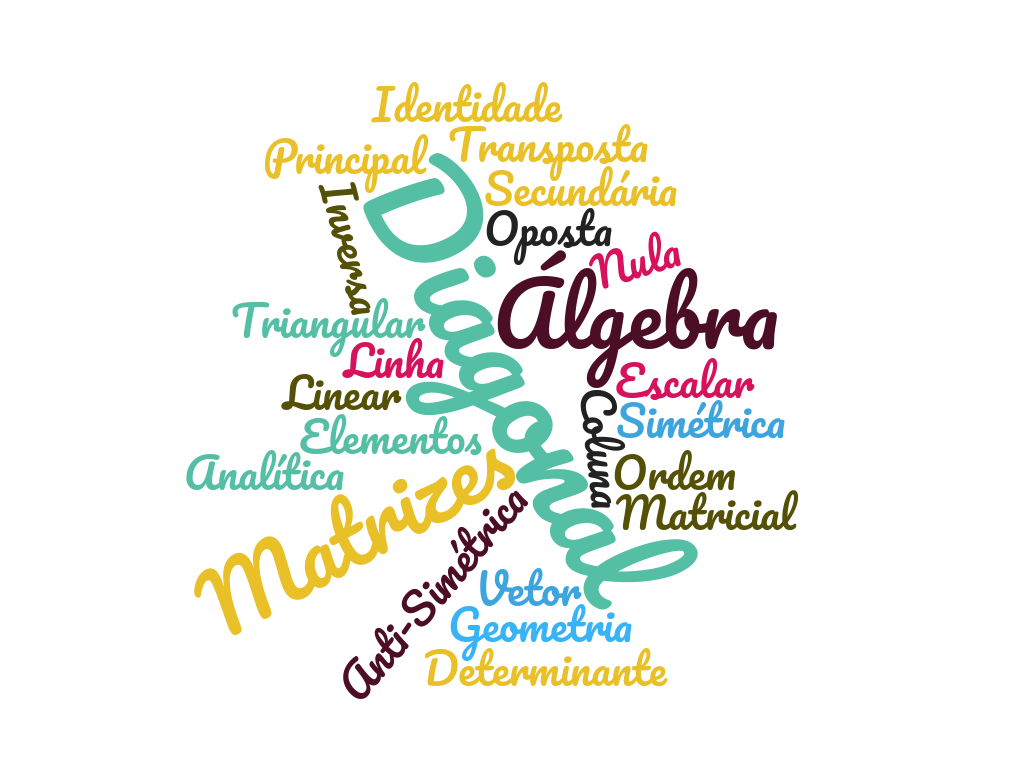
\includegraphics[scale=0.4]{linear_algebra.png}}
\end{center}
\end{figure}

\vspace{1cm}

\begin{center}
\textit{\textbf{\Large%
--- Desafio 2: Previsão do Tempo ---\\
\ \\
Abril/2019}}
\end{center}

%\vspace{1cm}
%\begin{flushright}
%\textbf{Monitor(es):}\\
%\textit{Monitor 1\\
%Monitor 2}
%\end{flushright}

%\begin{center}
%  \fbox{\fbox{\parbox{5.5in}{\centering
%        Answer the questions in the spaces provided on the
%        question sheets. If you run out of room for an answer,
%        continue on the back of the page.}}}
%\end{center}

\end{coverpages}




\newpage
%%%%%%%%%%%%%%%%%%%%%%%%%%%%%%%%%%%%%%%%%%%%%%%%%%%%%%%%%%%%%%%%%%%%%%%%%%%%%%%%%
%%%%%%%%%%%%%%%%%%%%%%%%%%%%%%%%%%%%%%%%%%%%%%%%%%%%%%%%%%%%%%%%%%%%%%%%%%%%%%%%%
%%%%%%%%%%%%%%%%%%%%%%%%%%%%%%%%%%%%%%%%%%%%%%%%%%%%%%%%%%%%%%%%%%%%%%%%%%%%%%%%%
\fullwidth{\section{Introdução}}
%\ifprintanswers
%\newpage
%\else
%\newpage
%\fi

O desafio agora é fazer uma previsão do tempo usando
um modelo bem simples de um Processo de Markov. Esse exercício
demonstrará o uso da álgebra linear na
resolução de um \emph{sistema de equações lineares} (que é a matéria da
Unidade 2 da disciplina).

Na tabela abaixo temos um modelo bem simples de previsão do
tempo\footnote{Este exemplo foi retirado do curso ``\ingles{Linear
    Algebra: Foundations to Frontiers (LAFF)''}, da The University of
  Texas at Austin, disponível em \url{http://www.ulaff.net}. Uma
  versão para estudo individual também está disponível na edX (\url{https://www.edx.org}).}.
O foco aqui não é se esse modelo é bom ou ruim, o foco aqui é demonstrar
que esse modelo é um exemplo bem simplificado de um Processo de Markov
que pode ser resolvido por álgebra linear para predizer o tempo.

\begin{table}[H]
  \centering
\begin{tabular}{cl|c|c|c|}
\cline{3-5}
\multicolumn{1}{l}{}                                   &         & \multicolumn{3}{c|}{\textbf{Hoje}} \\ \cline{3-5} 
\multicolumn{1}{l}{}                                   &         & Sol      & Nublado     & Chuva     \\ \hline
\multicolumn{1}{|c|}{\multirow{3}{*}{\textbf{Amanhã}}} & Sol     & 0.4      & 0.3         & 0.1       \\ \cline{2-5} 
\multicolumn{1}{|c|}{}                                 & Nublado & 0.4      & 0.3         & 0.6       \\ \cline{2-5} 
\multicolumn{1}{|c|}{}                                 & Chuva   & 0.2      & 0.4         & 0.3       \\ \hline
\end{tabular}
\end{table}

Nossa previsão do tempo baseia-se no seguinte fato: é possível saber a
probabilidade que o tempo \emph{amanhã} seja sol, nublado ou chuva,
dependendo se hoje está sol, nublado ou chuva. Isso está ilustrado na
tabela acima da seguinte maneira: se hoje é chuva, a probabilidade de
que amanhã seja nublado será de $0.6$ ($60\%$).


\begin{questions}
\setlength\linefillthickness{0.2pt}
%%%%%%%%%%%%%%%%%%%%%%%%%%%%%%%%%%%%%%%%%%%%%%%%%%%%%%%%%%%%%%%%%%%%%%%%%%%%%%%%%
%%%%%%%%%%%%%%%%%%%%%%%%%%%%%%%%%%%%%%%%%%%%%%%%%%%%%%%%%%%%%%%%%%%%%%%%%%%%%%%%%
%%%%%%%%%%%%%%%%%%%%%%%%%%%%%%%%%%%%%%%%%%%%%%%%%%%%%%%%%%%%%%%%%%%%%%%%%%%%%%%%%
\fullwidth{\section{Perguntas Fáceis}}

\question
Se hoje está nublado, qual a probabilidade de que amanhã seja sol?
\begin{solutionorlines}[0.25in]
  $0.3$
\end{solutionorlines}

\question
Se hoje está nublado, qual a probabilidade de que amanhã seja nublado?
\begin{solutionorlines}[0.25in]
  $0.3$
\end{solutionorlines}

\question
Se hoje o tempo é de chuva, qual a probabilidade de que amanhã seja
sol?
\begin{solutionorlines}[0.25in]
  $0.1$
\end{solutionorlines}


%%%%%%%%%%%%%%%%%%%%%%%%%%%%%%%%%%%%%%%%%%%%%%%%%%%%%%%%%%%%%%%%%%%%%%%%%%%%%%%%%
%%%%%%%%%%%%%%%%%%%%%%%%%%%%%%%%%%%%%%%%%%%%%%%%%%%%%%%%%%%%%%%%%%%%%%%%%%%%%%%%%
%%%%%%%%%%%%%%%%%%%%%%%%%%%%%%%%%%%%%%%%%%%%%%%%%%%%%%%%%%%%%%%%%%%%%%%%%%%%%%%%%
\fullwidth{\section{Perguntas Moderadamente Difíceis}}

\question
Se hoje está sol, qual a probabilidade de que o tempo \emph{depois de
  amanhã} seja de sol?
\begin{solutionorlines}[0.25in]
  $0.3$
\end{solutionorlines}

\question
Se hoje está sol, qual a probabilidade de que o tempo \emph{depois de
  amanhã} seja nublado?
\begin{solutionorlines}[0.25in]
  $0.4$
\end{solutionorlines}

\question
Se hoje está sol, qual a probabilidade de que o tempo \emph{depois de
  amanhã} seja de chuva?
\begin{solutionorlines}[0.25in]
  $0.3$
\end{solutionorlines}

\question
Este desafio utiliza um Processo de Markov para ilustrar como podemos utilizar
álgebra linear para prever o tempo utilizando um sistema de equações
lineares. Mas afinal: o que é um Processo de Markov\footnote{Sim, você
pode pesquisar na Wikipedia. Procure por \emph{Markov Chain}.}?
\begin{solutionorlines}[0.75in]
  Um processo de Markov (ou, melhor dizendo, uma \emph{Cadeia de
    Markov}) é um processo probabilístico com \emph{estados discretos}
  com a propriedade de que \emph{a
  distribuição de probabilidade para o próximo estado depende apenas
  do estado atual}, e não da cadeia de estados que o precederam. Essa
  propriedade é dita Markoviana.

  No nosso exemplo os estados discretos são ``sol'', ``nublado'' e
  ``chuva''. E a probabilidade para o próximo estado (por exemplo,
  amanhã) depende apenas da probabilidade do estado atual (``se hoje é
  sol'').
\end{solutionorlines}

%%%%%%%%%%%%%%%%%%%%%%%%%%%%%%%%%%%%%%%%%%%%%%%%%%%%%%%%%%%%%%%%%%%%%%%%%%%%%%%%%
%%%%%%%%%%%%%%%%%%%%%%%%%%%%%%%%%%%%%%%%%%%%%%%%%%%%%%%%%%%%%%%%%%%%%%%%%%%%%%%%%
%%%%%%%%%%%%%%%%%%%%%%%%%%%%%%%%%%%%%%%%%%%%%%%%%%%%%%%%%%%%%%%%%%%%%%%%%%%%%%%%%
\fullwidth{\section{Perguntas Difíceis}}

\fullwidth{Tente pensar pelo menos uns 10 minutos em como resolver
  essas questões. Talvez você não consiga pois ainda não estudou a
  unidade de sistemas de equações lineares na disciplina de álgebra,
  mas aqui vão algumas dicas: a) você precisa entender a tabela das
  probabilidades como um sistema de equações lineares; b) depois que
  você entendeu a tabela como um sistema de equações lineares, temos
  que representar essa tabela como uma matriz; e c) no final é muito
  fácil: basta multiplicar a matriz pelo vetor que representa a
  probabilidade do estado atual, ou seja, o tempo no dia de hoje.}

\question
Se hoje é segunda-feira e está nublado, qual é a probabilidade de que
na próxima segun\-da-feira (ou seja, daqui a 7 dias), o tempo seja sol?
\begin{solutionorlines}[0.25in]
  $0.3$
\end{solutionorlines}

\question
Se hoje é segunda-feira e está nublado, qual é a probabilidade de que
na próxima segun\-da-feira (ou seja, daqui a 7 dias), o tempo seja nublado?
\begin{solutionorlines}[0.25in]
  $0.3$
\end{solutionorlines}

\question
Se hoje é segunda-feira e está nublado, qual é a probabilidade de que
na próxima segun\-da-feira (ou seja, daqui a 7 dias), o tempo seja de chuva?
\begin{solutionorlines}[0.25in]
  $0.3$
\end{solutionorlines}

%% \question
%% Questão
%% \ifprintanswers
%% \begin{solution}
%% \begin{parts}
%%   \part ``pergunta''.\\
%%   $=$ \emph{resposta}
%%   \part ``pergunta''\\
%%   $=$ \emph{resposta}
%%   \part ``pergunta''.\\
%%   $=$ \emph{resposta}
%% \end{parts}
%% \end{solution}
%% \else
%% \begin{parts}
%%   \part ``pergunta''.
%%   \umalinha
%%   \part ``pergunta''
%%   \umalinha
%%   \part ``pergunta''.
%%   \umalinha
%% \end{parts}
%% \fi

%% \question
%% Pergunta
%% \begin{checkboxes}
%%   \choice resp
%%   \choice resp
%%   \choice resp
%%   \CorrectChoice respcorreta
%% \end{checkboxes}

%% \question
%% Relacione os números
%% \begin{enumerate}
%% \item resp 1
%% \item resp 2
%% \item resp 3
%% \item resp 4
%% \item resp 5
%% \item resp 6
%% \end{enumerate}
%% \begin{parts}
%%   \part \vf[5] frase
%%   \part \vf[2] frase
%%   \part \vf[1] frase
%%   \part \vf[6] frase
%%   \part \vf[4] frase
%%   \part \vf[3] frase
%% \end{parts}

%% \question
%% Pergunta
%% \ifprintanswers
%% \begin{solution}
%% \begin{enumerate}
%%   \item item
%%   \item item
%%   \item item
%%   \item item
%%   \item item
%%   \item item
%%   \item item
%% \end{enumerate}
%% \end{solution}
%% \else
%% \begin{enumerate}
%%   \item \_\_\_\_\_\_\_\_\_\_\_\_\_\_\_\_\_\_\_\_\_\_\_\_\_\_\_\_\_\_\_\_\_\_\_\_\_\_\_\_\_\_\_\_\_\_\_\_\_\_\_\_\_\_\_\_
%%   \item \_\_\_\_\_\_\_\_\_\_\_\_\_\_\_\_\_\_\_\_\_\_\_\_\_\_\_\_\_\_\_\_\_\_\_\_\_\_\_\_\_\_\_\_\_\_\_\_\_\_\_\_\_\_\_\_
%%   \item \_\_\_\_\_\_\_\_\_\_\_\_\_\_\_\_\_\_\_\_\_\_\_\_\_\_\_\_\_\_\_\_\_\_\_\_\_\_\_\_\_\_\_\_\_\_\_\_\_\_\_\_\_\_\_\_
%%   \item \_\_\_\_\_\_\_\_\_\_\_\_\_\_\_\_\_\_\_\_\_\_\_\_\_\_\_\_\_\_\_\_\_\_\_\_\_\_\_\_\_\_\_\_\_\_\_\_\_\_\_\_\_\_\_\_
%%   \item \_\_\_\_\_\_\_\_\_\_\_\_\_\_\_\_\_\_\_\_\_\_\_\_\_\_\_\_\_\_\_\_\_\_\_\_\_\_\_\_\_\_\_\_\_\_\_\_\_\_\_\_\_\_\_\_
%%   \item \_\_\_\_\_\_\_\_\_\_\_\_\_\_\_\_\_\_\_\_\_\_\_\_\_\_\_\_\_\_\_\_\_\_\_\_\_\_\_\_\_\_\_\_\_\_\_\_\_\_\_\_\_\_\_\_
%%   \item \_\_\_\_\_\_\_\_\_\_\_\_\_\_\_\_\_\_\_\_\_\_\_\_\_\_\_\_\_\_\_\_\_\_\_\_\_\_\_\_\_\_\_\_\_\_\_\_\_\_\_\_\_\_\_\_
%% \end{enumerate}
%% \fi


%%%%%%%%%%%%%%%%%%%%%%%%%%%%%%%%%%%%%%%%%%%%%%%%%%%%%%%%%%%%%%%%%%%%%%%%%%%%%%%%%
%%%%%%%%%%%%%%%%%%%%%%%%%%%%%%%%%%%%%%%%%%%%%%%%%%%%%%%%%%%%%%%%%%%%%%%%%%%%%%%%%
%%%%%%%%%%%%%%%%%%%%%%%%%%%%%%%%%%%%%%%%%%%%%%%%%%%%%%%%%%%%%%%%%%%%%%%%%%%%%%%%%
%%%%%%%%%%%%%%%%%%%%%%%%%%%%%%%%%%%%%%%%%%%%%%%%%%%%%%%%%%%%%%%%%%%%%%%%%%%%%%%%%
%%%%%%%%%%%%%%%%%%%%%%%%%%%%%% TERMINA O DOCUMENTO %%%%%%%%%%%%%%%%%%%%%%%%%%%%%%
%%%%%%%%%%%%%%%%%%%%%%%%%%%%%%%%%%%%%%%%%%%%%%%%%%%%%%%%%%%%%%%%%%%%%%%%%%%%%%%%%
%%%%%%%%%%%%%%%%%%%%%%%%%%%%%%%%%%%%%%%%%%%%%%%%%%%%%%%%%%%%%%%%%%%%%%%%%%%%%%%%%
%%%%%%%%%%%%%%%%%%%%%%%%%%%%%%%%%%%%%%%%%%%%%%%%%%%%%%%%%%%%%%%%%%%%%%%%%%%%%%%%%
%%%%%%%%%%%%%%%%%%%%%%%%%%%%%%%%%%%%%%%%%%%%%%%%%%%%%%%%%%%%%%%%%%%%%%%%%%%%%%%%%
\end{questions}
\end{document}
